
\chapter{Results} % Main chapter title

\label{Chapter4} % For referencing the chapter elsewhere, use \ref{Chapter1} 

\lhead{Chapter 4. \emph{Results}} % This is for the header on each page - perhaps a shortened title

%----------------------------------------------------------------------------------------
\setstretch{1}
\section{System Inputs}
Using the Figure \ref{fig:phantom} as the input phantom image, all the resulted reconstructed images were obtained with the image reconstruction algorithm as described in the chapter 2.  

\begin{figure}[H]
	\centering
		
\includegraphics[width=150pt]{Figures/Sl.png}
	\caption[Input Phantom Image.]{Shepp-Logan Phantom Image.}
	\label{fig:phantom}
\end{figure}
%----------------------------------------------------------------------------------------

This software allows user to select the size of the image to be constructed in the run time. For a instance, 

\begin{verbatim}
Please input the image file number to be constructed: 
 1 - Shepp_Logan image with size 256 x 256
 2 - Shepp_Logan image with size 200 x 200
 3 - Shepp_Logan image with size 100 x 100
Your choice: 1
\end{verbatim}
As a system constrained, we always use square, even size gray-scale  PGM ASCII image format. 

Then the user has to input the required X-ray beam spacing that will be used to perform the radon transform. As a user guidance, this software system will provide minimum beam spacing if the user really wants to use the maximum number of beams for the reconstruction process.

As the next inputs, user has to select the type of the filter and the interpolation method that he/she wants to apply on the image. For a instance, 
\begin{verbatim}
Please input the type of the Filter: 
 1 : Shepp-Logan filter
 2 : Ram-Lak filter 
 3 : Low-pass cosine filter 
Your choice: 1
 
Please input the type of the Interporlator: 
 1 : Linear Interpolator
 2 : Nearest neighbor Interpolator 
Your choice: 1
\end{verbatim}

After that the system will generate and store the corresponding reconstructed image along with the Radon transform image and the convolution image inside the main folder. User can compare the output image with the original image stored inside the Phantom folder.   

\section{System Outputs}
According to the above input parameters, we can see that there are different possible combinations that user can use while executing the system. But here we are going to consider only few important test cases. 

\subsection{Test case 1:}
\begin{itemize}
\item Image size: $256 \times 256$
\item Beam spacing: 0.005 (i.e 363 beams)
\item Filter: Shepp-Logan
\item Interpolator:  Linear 
\end{itemize}

\paragraph{Radon Transformation}
The output of the radon transformation for the test case 1 is shown in the Figure \ref{fig:radont1}.  
\begin{figure}[H]
	\centering
		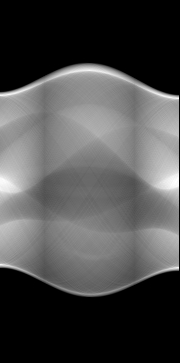
\includegraphics[width=80pt]{Figures/RadonTransform256.jpg}
	\caption[Radon transform of test case 1.]{Radon transform of test case 1.}
	\label{fig:radont1}
\end{figure}

\paragraph{Convolution}
The output of the convolution (i.e. filtered Radon transformation) for the test case 1 is shown in the Figure \ref{fig:cont1}.  
\begin{figure}[H]
	\centering
		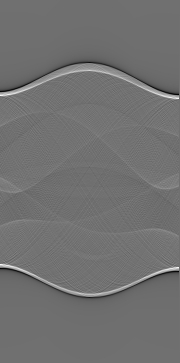
\includegraphics[width=80pt]{Figures/Convolution256.jpg}
	\caption[Convolution of test case 1.]{Convolution of test case 1.}
	\label{fig:cont1}
\end{figure}

\paragraph{Back projection Transformation}
Corresponding reconstructed image is given by the Figure \ref{fig:t1}.  
\begin{figure}[H]
	\centering
		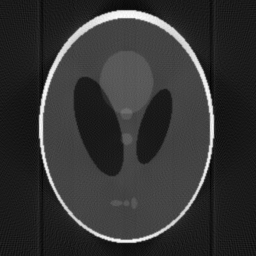
\includegraphics[width=150pt]{Figures/ReconstructedImage256.jpg}
	\caption[Test case 1 image.]{Test case1: Reconstructed phantom.}
	\label{fig:t1}
\end{figure}

The error related to the above reconstruction is given by the Figure \ref{fig:error}.  
\begin{figure}[H]
	\centering
		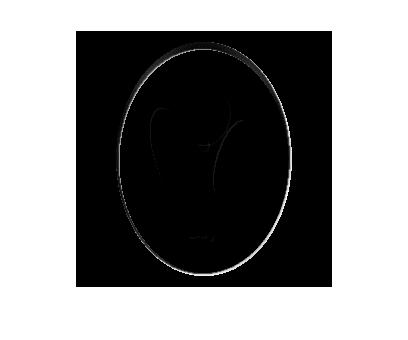
\includegraphics[width=230pt]{Figures/error.jpg}
	\caption[Reconstruction error image.]{Error of test case 1.}
	\label{fig:error}
\end{figure}

According to the error image \ref{fig:error}, we can conclude that the most of intensity errors occurred only near the edges of the phantom image.




\subsection{Test case 2:}
\begin{itemize}
\item Image size: $256 \times 256$
\item Beam spacing: 0.02 (i.e 121 beams)
\item Filter: Shepp-Logan
\item Interpolator:  Linear 
\end{itemize}
Corresponding reconstructed image is given by the Figure \ref{fig:t2}.  
\begin{figure}[H]
	\centering
		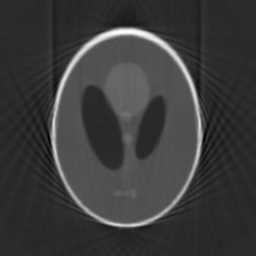
\includegraphics[width=150pt]{Figures/ReconstructedImage256t2.jpg}
	\caption[Test case 2 image.]{Test case2: Reconstructed phantom.}
	\label{fig:t2}
\end{figure}
According to the output image \ref{fig:t2}, we can see that the image become little blurred and distorted with respect to the Figure \ref{fig:t1}. This is because, for test case 2, we only used one third of beams compared to the test case 1. But this process is much faster than test case 1 process. 

Similar to this test cases, user can reconstruct image using different interpolators and filters provide by this system. 

\section{Performance Analysis }
From our experience the linear interpolator with the Shepp-logan filter or Low pass cosine filter will give the best result of the image reconstruction. Therefore in the following we will analyze the result using the linear interpolator and Shepp-logan filter setting for the code.

\begin{table}[htp]
\centering
\begin{tabular}{|c |c| c |c |}
 \hline
 \multicolumn{2}{|c|}{[1] main.cpp }& \multicolumn{2}{|c|}{ time = 14.1911 } \\
 \hline
subroutine & Time Percentage & total time & loops \\
 \hline
[6] Radon Transformation & $0.9\%$ & 0.1225 & 1\\
  \hline
[2] Image Reconstruction &  $70.1\%$ & 9.9471 & 1\\
 \hline
  \multicolumn{2}{|c|}{[2] Image Reconstuction }& \multicolumn{2}{|c|}{time = 9.9471} \\
 \hline
subroutine & Time Percentage & total time & loops \\
 \hline
[3] Back Projection & $99.8\%$ & 9.9236 & 1\\
  \hline
[7] Convolution &  $0.2\%$ & 0.0235 & 1\\
 \hline
   \multicolumn{2}{|c|}{[3] Back Projection  }& \multicolumn{2}{|c|}{time = 14.0130} \\
 \hline
 subroutine & Time Percentage & total time & loops \\
 \hline
[4] Summation over $\theta$ & $96.2\%$ & 9.5455 & 65536\\
  \hline
[8] Linear Index &  $0.0\%$ & 0.001 & 65536\\
 \hline
   \multicolumn{2}{|c|}{[4] Summation over $\theta$  }& \multicolumn{2}{|c|}{time = 9.5455} \\
 \hline
 subroutine & Time Percentage & total time & loops \\
 \hline
[5] Linear Interpolation & $92.1\%$ & 8.7874 & 11796480\\
  \hline
[8] Calculation of t &  $6.571\%$ & 0.6270 & 11796480\\
 \hline
    \multicolumn{2}{|c|}{[5] Linear Interpolation  }& \multicolumn{2}{|c|}{time = 8.7874} \\
 \hline
 subroutine & Time Percentage & total time$^*$ & loops \\
 \hline
[5] tent & $30.4\%$ & 2.671 & 4282122240\\
  \hline
[8] Linear Index &  $45.3\%$ & 3.984 & 4282122240\\
 \hline
\end{tabular}
\caption{Time table for main.exe for image of 256 x 256 and the beam spacing is chosen as d=0.007. Shepp-logan filter and linear interpolator are used in this run. Notice that in the subroutine of Linear Interpolator only the precentage is measured by Timer. The time inside this subroutine is calculated from the precentage of total time.}\label{table1}
\end{table}

The results from timer are in shown in the time Table.\ref{table1}. From this figure it is easy to notice that most of the time is cost in the back projection part. Because there are three loops inside the back projection and the interpolation is called 11796480 times in order to do the back projection for output figure with 256x256 pixels. Most of the time are cost inside these loops. In order to optimize the code we already used the linear index to access the element of all the RectMDArray objects. It is shown in the table that linear index has the same order of time consume with other flop operation. All function asr actually made in line since we used -o3 option in the compiler and we inline all possible member functions inside interpolator class. Therefore the only way to optimize the code is to parallelize the back projection because the back projection are independent with each other and the loops inside it is most time consuming.

The timer class has a bug in it which it could allow use the timer inside another timer and by including it inside the inner loops of interpolator class it really slow down the code into 100 seconds. Because there are too many loops here timer in the most inside loop will definitely slow down the code. Therefore in the most inner subroutine we use the timer to calculate the percentage of each function but calculate the real time by multiply the percentage with the total time of the parent subroutine.
